%%%%%%%%%%%%%%%%%%
% skybox

\section{Skybox}

Skybox je vzdálené okolí od scény, které nereprezentujeme pomocí polygonů, ale jen pomocí obrázků.
Skybox můžeme použít pro reprezentaci mraků, vzdálených krajů nebo třeba hvězd ve vesmíru.
Obvykle bývá skybox ve formě krychle.
Na všechny stěny krychle je nanesen jiný obrázek.
Obrázky na sebe navazují a tvoří tak dojem okolí.
Příklad roz\-vi\-nu\-té\-ho krychlového skyboxu můžeme vidět na obrázku: \ref{fig:skybox0}.
Skybox můžeme vytvořit fotoaparátem a programem na skládání fotografií.
Stačí vyfotit okolí ve všech směrech a fotografie následně složit dohromady.
V našem případě si ale musíme skybox vygenerovat.
V práci budeme používat dvě metody generování skyboxu.
\begin{figure}[h]
\centering
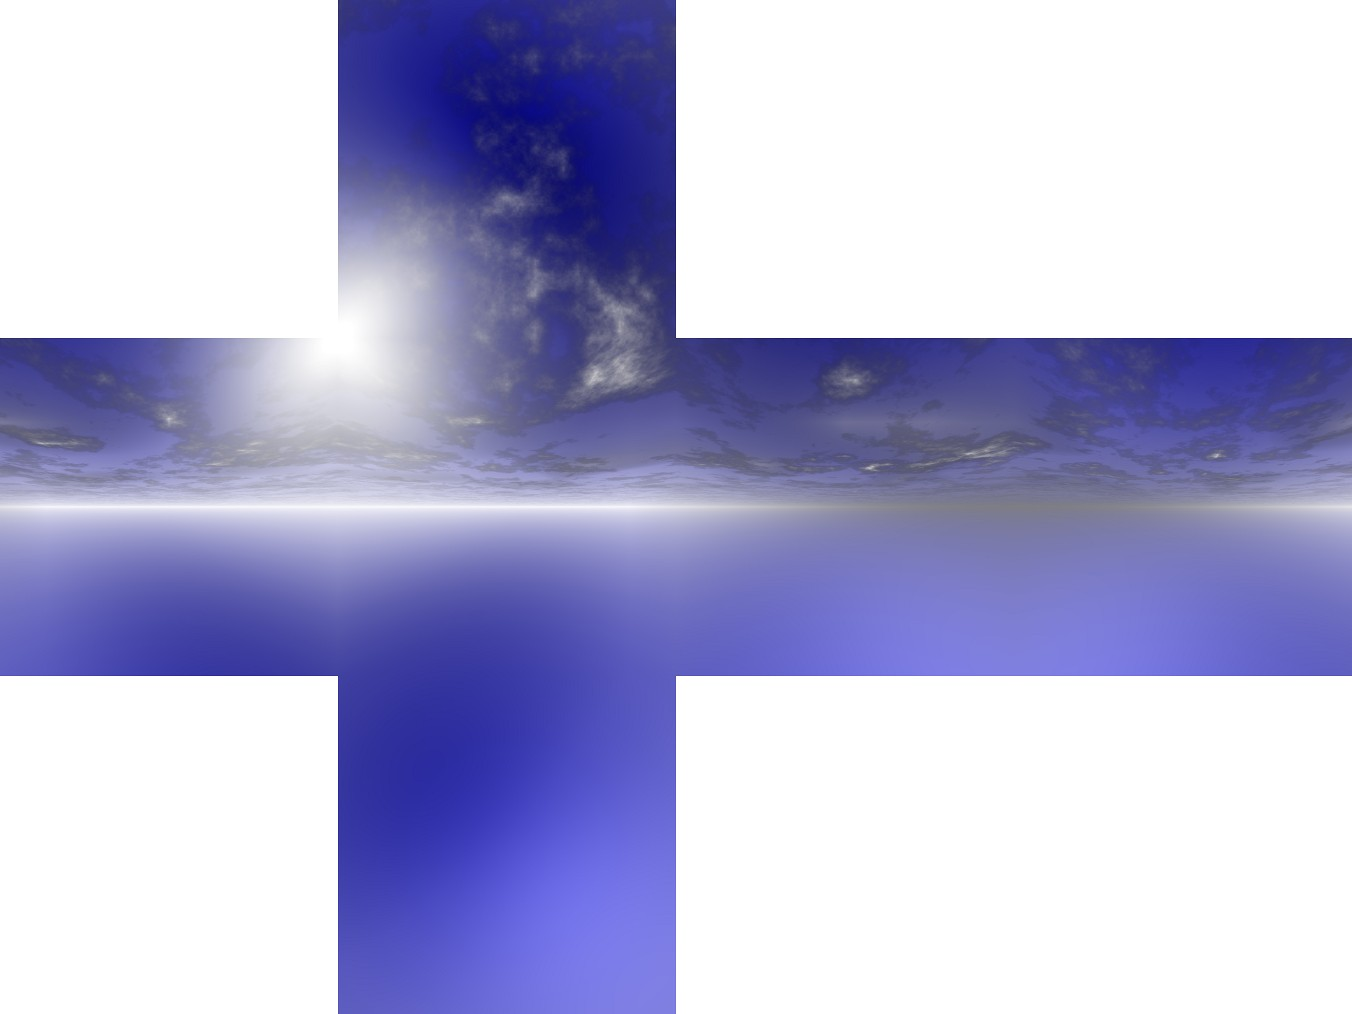
\includegraphics[width=15cm,keepaspectratio]{obr/skybox0.jpg}
\caption{Skybox zobrazující dopolední oblohu}
\label{fig:skybox0}
\end{figure}


První je obdobná tvorbě skyboxu pomocí fotoaparátu.
Z jednoho vybraného místa si scénu vykreslíme do šesti směrů a výsledky si uložíme.
Zorný uhel kamery nastavíme na $90$ stupňů a šířku a výšku vykreslené oblasti zvolíme totožnou.
Tímto dokážeme vytvořit jednoduché skyboxy. V práci budeme takto vytvořený skybox používat pro odraz na hladině vody.
Na složitější skybox (například oblohy) tato metoda ale nestačí.

Druhá metoda vykresluje stěny skyboxu zároveň.
Metodu budeme využívat pro oblohy.
Ze středu krychle se pro zvolený pixel a zvolenou stěnu krychle určí paprsek.
Pro velikost obrázků na stěnách krychle $(w,h)$ potřebujeme $6 \cdot w \cdot h$ paprsků.
Paprsek můžeme reprezentovat pouze normalizovaným vektorem $u$.
Tento vektor si můžeme představit jako jistou třísložkovou souřadnici.
Pokud budeme chtít vykreslit do skyboxu jistý element, předáme mu tento vektor a element nám vrátí barvu $(r,g,b,a)$.
Číslo $a$ je průhlednost v intervalu $\langle 0,1 \rangle$ a používá se pro míchání nově příchozí barvy $c=(r,g,b)$ s předcházející $cp=(r_p,g_p,b_p)$.
Míchání je řízeno vztahem:
\begin{equation}
cp=a \cdot c + (1-a) \cdot cp
\end{equation}
Algoritmus generování skyboxu obohy je následující:
\begin{enumerate}
\item Nastavíme všechny barvy obrázků na nulu $cp=(0,0,0)$.
\item Pro všechny stěny krychle skyboxu a všechny jejich pixely určíme normalizovaný vektor $u$.
\item Pro všechny elementy $e_i, i \in {1,\dotsc,n}$, které chceme vykreslit získáme barvu $c_i$.
\item Výsledná barva pro vektor $u$ (a tedy i pro konkrétní pixel) je $cp_n$.
\begin{eqnarray*}
\label{eq:fastindex}
cp_{1}   &=& a_{1} \cdot c_{1} + (1-a_1) \cdot cp     \\
cp_{i} &=& a_{i} \cdot c_{i} + (1-a_i) \cdot cp_{i-1}
\end{eqnarray*}
\end{enumerate}

Oblohu si budeme reprezentovat pomocí tři základní elementů:

\begin{itemize}
\item Barevný přechod oblohy.
Barevný přechod oblohy udává barvu pozadí.
Udává barvu atmosféry při východu slunce, západu slunce nebo v průběhu odpoledne.
Barevný přechod je určen barvou horizontu, počáteční, koncovou a základní barvou, vektorem ke slunci a exponentem.
Počáteční barva oblohy je barva blízko slunce, koncová barva oblohy je barva na opačném konci oblohy od slunce.
Základní barva je barva mezi počáteční a koncovou.
Barva horizontu obarvuje oblohu blízko nad zemí.
Rozmístění barev je dobře patrné na obrázku \ref{fig:skyboxgrad}
Exponent udává rychlost změny barvy horizontu do barvy oblohy.
\begin{figure}[h]
\centering
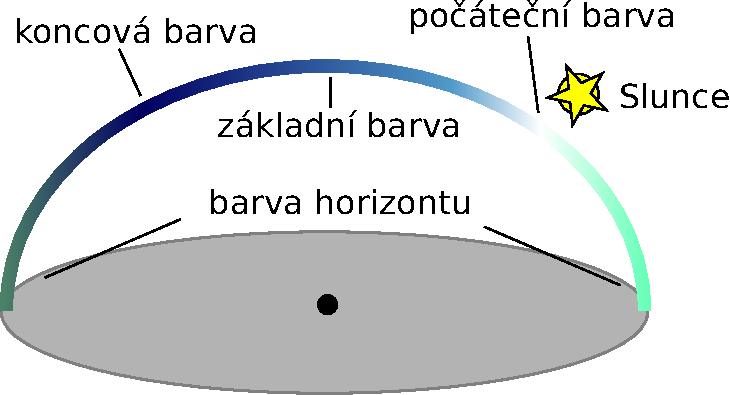
\includegraphics[width=7.5cm,keepaspectratio]{obr/skyboxgrad.pdf}
\caption{Rozmístění barev oblohy.}
\label{fig:skyboxgrad}
\end{figure}

\item Slunce.
Slunce je určeno vektorem pozice, velikostí, barvou, exponentem a velikostí okolní záře.
Velikost slunce je ve steradiánech.
Exponent udává, jak ostrá je hranice slunce.
Velikost okolní záře udává, do jaké vzdálenost od slunce se šíří barva slunce obrázek: \ref{fig:skyboxsun}.
\begin{figure}[h]
\centering
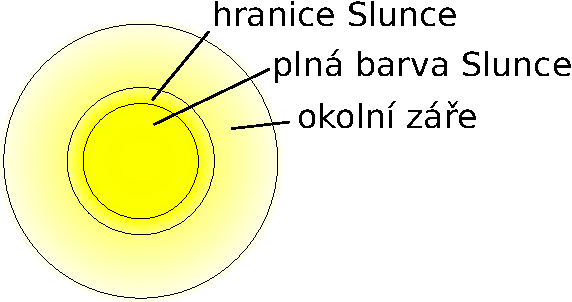
\includegraphics[width=7.5cm,keepaspectratio]{obr/skyboxsun.pdf}
\caption{Hranice slunce a okolní záře.}
\label{fig:skyboxsun}
\end{figure}

\item Mraky.
Mraky jsou reprezentované nekonečnou rovinou, která je umístěna nad scénou, obrázek: \ref{fig:skyboxcloud}.
Směrový vektor $u$ pro daný pixel skyboxu protne tuto rovinu v jistých souřadnicích $I(x,y)$.
Souřadnice $I$ použijeme jako vstup funkce Perlinova šumu popsaného v podsekci \ref{subsec:perlin}.
Parametry mraků jsou tedy: Amplituda, frekvence, perzistence a počet sčítání.
Tyto parametry jsou předány funkci Perlinova šumu.
Další parametry jsou hustota, krytí a barva mraků.
Pro věrnější reprezentaci mraků budeme obvykle potřebovat vícero vrstev mraků.
Problém teto metody spočívá v aliasing efektu na horizontu.
Průsečík směrového vektoru s rovinou mraků je pro pixely na horizontu velmi daleko.
Jednotlivé souřadnice pro Perlinův šum pro pixely, které leží vedle sebe v této oblasti jsou velmi odlišné.
Tím nám vzniká problém, že barva mraků na horizontu se prudce střídá v sousedních pixelech.
Řešení by mohlo spočívat v použití jiného než Perlinova šumu.
Naším řešením ale bude zvyšování průhlednosti mraků směrem k horizontu.
Mraky se tak rozplynou v barvě horizontu, obrázek: \ref{fig:cloudalias}.
\begin{figure}[h]
\centering
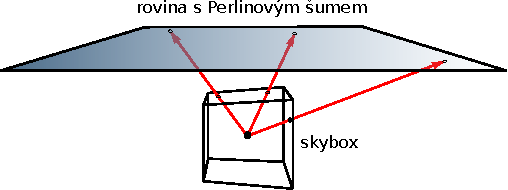
\includegraphics[width=7.5cm,keepaspectratio]{obr/skyboxcloud.pdf}
\caption{Vykreslování mraků.}
\label{fig:skyboxcloud}
\end{figure}

\begin{figure}[h]
\centering
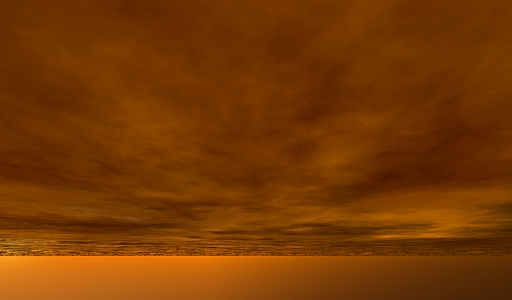
\includegraphics[width=7.5cm,keepaspectratio]{obr/skyboxalias.jpg}
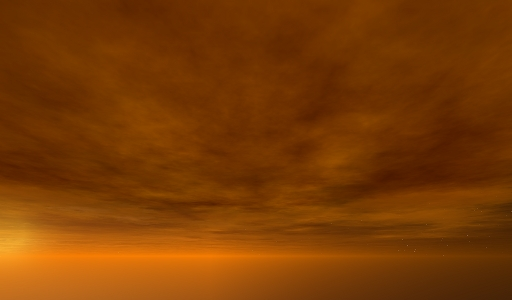
\includegraphics[width=7.5cm,keepaspectratio]{obr/skyboxantialias.jpg}
\caption{Vlevo: mrak bez opravy aliasing efektu. Vpravo: mrak s rostoucí průhledností k horizontu.}
\label{fig:cloudalias}
\end{figure}


\end{itemize}

\begin{figure}[h]
\centering
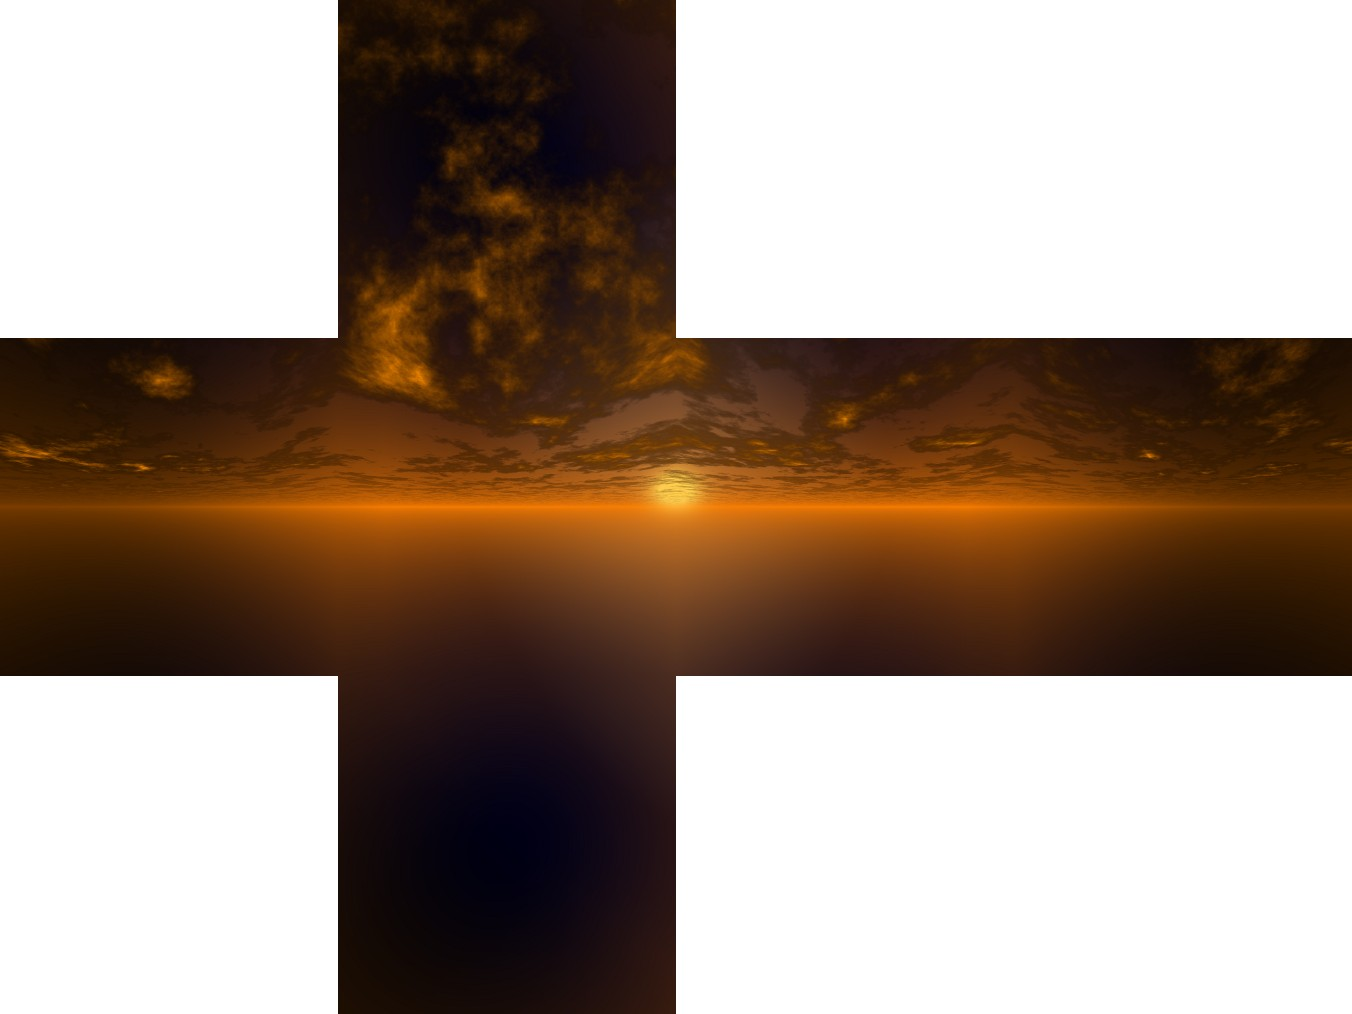
\includegraphics[width=15cm,keepaspectratio]{obr/skybox1.jpg}
\caption{Skybox zobrazující západ slunce}
\label{fig:skybox1}
\end{figure}






